\documentclass[12pt]{article}
\usepackage{hyperref}
\usepackage{graphicx}
	\begin{document}

		\begin{titlepage}

			\newcommand{\HRule}{\rule{\linewidth}{0.5mm}}
			\center
 
			\textsc{\LARGE Cardiff University}\\[1.5cm] 
			\textsc{\Large CM3106 Multimedia}\\[0.5cm] 

			\HRule \\[0.4cm]
				{ \huge \bfseries MATLAB Interactive Fourier-based Synthesiser}\\[0.4cm] 
			\HRule \\[1.5cm]
 
			\begin{minipage}{0.4\textwidth}
				\begin{flushleft} \large
					\emph{Student Name:}\\
						Geraint \textsc{Harries} \newline
					\emph{Student Number:}\\
						1100682
				\end{flushleft}
			\end{minipage}
			~
			\begin{minipage}{0.4\textwidth}
				\begin{flushright} \large
					\emph{Lecturer(s):} \\
						Prof. David \textsc{Marshall} \\
						Dr. Kirill \textsc{Sidorov}
				\end{flushright}
			\end{minipage}\\[4cm]

			{\large \today}\\[3cm] 

			\vfill 

		\end{titlepage}
		
		\section{Program Overview}

			This program is inspired by a piece of audio software called Iris by Izotope Inc. I have used this software as inspiration. I am able to load audio and graphically represent and edit the time-frequency distrubution. I am also able to apply other audio effects such as Tromolo, Ring Modulation, Wah Wah etc as well as volume shaping. Many of the variables for each audio effect are modifiable by the user. Below is a description of the basic algorithm design and main elements of each section of my program. There are also detailed comments within the code.   

		\section{Algorithm List and Description}
			
			\subsection{Reading in an audio input file}
				 This function allows the user to select an audio file from thier directory and save the frequency and file as global variables \textsc{wavefrequency} and \textsc{wavefile} respectivly.

			\subsection{Compute Fourier}
			
				This function computes and shows the short term fourier transform of an audiofile.\newline 

				The Pseudocode:

				\begin{itemize}
  					\item Get short term fourier transform of the audio file.
    					\item Convert the complex magnitude of the fourier transform into absolute values.
      					\item Show the output and save to a variable. 
      				\end{itemize}

			\subsection{Volume Shaping}

				This function generates a basic volume shaping on an audio file. It does so by generating a graph of a basic ADSR shape (Shown in Figure 1) and then calculating the dot product of the ADSR and audio file. 

				\begin{figure}[h!]
  					\centering
            				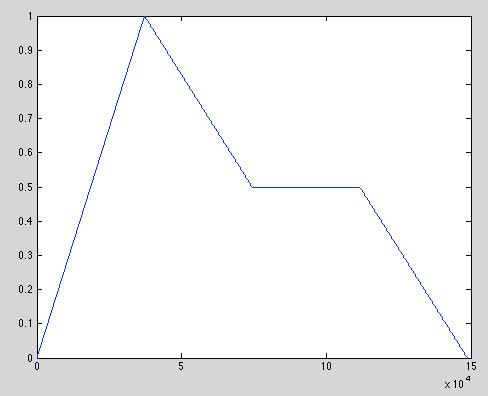
\includegraphics[width=7cm]{VolumeShaping.png}
	      				\caption{ADSR Schematic}
				\end{figure}

				The Pseudocode:

				\begin{itemize}
					\item Generate the ADSR graph.
					\item Calculate the dot product of the ADSR graph and the audio file.
					\item Return calculated value 
				\end{itemize}

			\subsection{Reverb}

			\subsubsection{Standard Reverb}

				This function generate a reverb effect on given audio given a users parameters. It adds this vector to the original audio file and then returns it. \\

				The Pseudocode:

				\begin{itemize}
					\item Generate a reverb vector by using the users gain and delay value.  
					\item The vector is added to the original audio file.
					\item Assign the calcuation to the audio file.
				\end{itemize}

			\subsubsection{Reverb Convolution}
				
				This function generates a reverb effect on given audio using another audio file the user has selected. It convolves the two audio files and normalizes the output to +-1.  \\
				The Pseudocode:

				\begin{itemize}
					\item Find smallest of two files
					\item Fast fourier transform both
					\item Calculate the dot product
					\item Inverse fast fourier transform the calculated dot product
					\item Return the first N (length of shortest) elements
				\end{itemize}

			\subsection{Wah Wah}
				
				This function runs the wah wah effect on the audio file. It does so by creating a variable peak response of a filter and applying it to the audio file.\newline

				The Pseudocode:

				\begin{itemize}
					\item Create empty vector same size as the audio file
					\item Iterating through each element in the vector calculate the value for the oscilating sine wave and add or remove it from the from the original file.
					\item Add it to the empty vector.
				\end{itemize}

			\subsection{Ring Modulation}

				This function allows the user to generate a ring modulation to their audio file. A carrier vector is created and then a dot product is calculated.\newline  
				
				The Pseudocode:

				\begin{itemize}
					\item Create a carier vector 
					\item Calculate the dot product of the carrier and audio file. 
					\item Assign dot product calculation to original audio file.
				\end{itemize}

			\subsection{Phase Vocoder}

				I have implemented two options for the user regarding phase vocoding. One uses user entered values, the user is able to specify the ratio by which the pitch increases (See Figure 2). The other is by using the GUI keyboard (See Figure 3). Both ways use the same algorithm. It generates a slower or faster file given a fraction (either the user supplies or which is pre-set). The audio file is then resampled using the same ratio. The ratios were found from url{http://oeis.org/DUNNE/TEMPERAMENT.HTML} \newline

				The Pseudocode:

				\begin{itemize}
					\item Generate ratio using either preset or user given numerator and denominator.
					\item Generate a changed speed audio file given the ratio 
					\item Resample the speed changed audio to the desired pitch given the ratio  
				\end{itemize}

				\begin{figure}[h!]
  					\centering
            				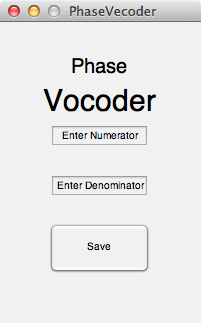
\includegraphics[width=5cm]{PhaseUserInput.png}
	      				\caption{User input for phase vocoder}
				\end{figure}
				\begin{figure}[h!]
					\centering
					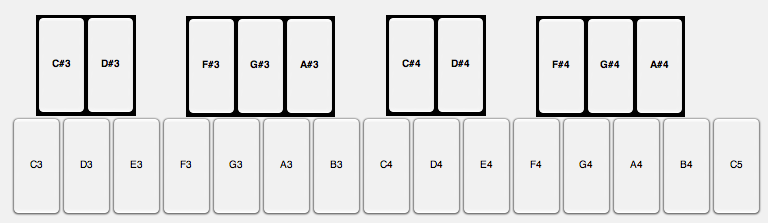
\includegraphics[width=14cm]{Keyboard.png}
					\caption{Keyboard with specific phase vecoded frequencies}
				\end{figure}

			\subsection{Save}

				This function saves the graphically audio file. The edit function does not save the file after editing as to allow the user the choice of whether to edit their change. It simply uses istft on the edited spectrogram and saves that to the global variable of the audio file.  

			\subsection{Edit}

				This function creates a mask with the same dimensions as the fourier transform of the audio file. Using imfreehand, it allows the user to draw on the transparent mask and then generates a binary image of the users drawing. A dot product is then generated of the binary image and spectrogram. The changed spectrogram is then displayed. N.B. The new spectrogram is not saved, it only saves if you press the save button.\newline

				The Pseudocode:

				\begin{itemize}
					\item Create and display transparent mask of same dimensions as fourier transform of audio file.
					\item Record the free hand drawing of the user
					\item Generate a binary mask from the drawing
					\item Calculate the dot product of the binary mask and fourier of original audio file.
				\end{itemize}

			\subsection{Tremolo}

				This function generates a tremolo effect given the users values for alpha and FC. It generates a tremolo vector and then calculates the dot product for the vector and original audio file. 

				\begin{itemize}
					\item Generate tremolo vector given user input of alpha and Fc
					\item Calculate the dot product of vector and original audio file
					\item Assign to original audio file
				\end{itemize}

			\subsection{AudioPlayer}
		
				I have implemented audioplayer which is able to do the following: 
				\begin{itemize}
					\item Play 
					\item Pause
					\item Stop
					\item Record
				\end{itemize}

			\subsection{Loop}

				I implemented looping by creating an infinite loop and outputting the file within it
			
			\subsection{Reverse}
			
				Using the flipud() MATLAB function, I was able to flip the audio file matrix. This essentially reversed the audio.

		\section{Novel Features}

			As previously mentioned in subsections 2.42, 2.11, 2.12 and 2.13, I implemented reverb convolution, recording, looping and reversing. These are my novel features as they are not strictly part of the core criteria (although reverb is, reverb convolution isn't). You wil see the detail of these features in the aforementioned subsections. There are also detailed comments within the code.  

		\section{Satisfying the basic criteria}

			I beleive that I satisfied all of the basic criteria of the coursework. I implemented:
			
			\begin{itemize}
				\item A method of reading in an input audio file (2.1)
				\item Computed its underlying time-frequency distribution (2.2)
				\item Provided an interactive means of editing this via its displayed spectrogram (2.8)
				\item The resulting audio is able to be played back (2.11, 2.7)
				\item New sounds are able to be generated using the interactive keyboard. (2.7)
				\item Volume Shaping to control the basic sounds produced (2.3)
				\item Tremolo (2.10)
				\item Wah Wah (2.5)
				\item Ring Modulation (2.6)
				\item Basic Reverb (2.4.1)
			\end{itemize}

			Given these functions I feel I have met the core requirements. I have also implemented 
			
			\begin{itemize}
				\item Reverb Convolution (2.4.2)
				\item The ability to record (2.11)
				\item The ability to loop audio (2.12)
				\item The ability to reverse audio. (2.13)
			\end{itemize}	

				These features were not part of the core requirement and therefor count as novel feature. Therefore, in that regard, I feel that I have meet all the criteria of this coursework including novel features. 

\end{document}
